%%%%%%%%%%%%%%%%%%%%%%%%%%%%%%%%%%%%%%%%%%%%%%%%%%%%%%%%%%%%%%%%%%%%%%%%%%%%%%%
% Chapter 4: HtmlForm renderer
%%%%%%%%%%%%%%%%%%%%%%%%%%%%%%%%%%%%%%%%%%%%%%%%%%%%%%%%%%%%%%%%%%%%%%%%%%%%%%%

%++++++++++++++++++++++++++++++++++++++++++++++++++++++++++++++++++++++++++++++

Este renderer permitir\'a generar un documento HTML5 con un formulario en el que se encuentran todas las
preguntas listas para ser completadas desde el navegador. Posee adem\'as todos los JavaScripts necesarios
para la correci\'on autom\'aticas de las mismas.
\bigskip

El objetivo de este renderer es proporcionar al alumno una serie de preguntas para que practique con vistas
a afrontar un examen oficial. La principal ventaja que ofrece es la portabilidad: al ser un documento HTML puede
alojarse en cualquier servidor o ejecutarse localmente desde un navegador sin tener que configurar nada previamente.
Solo es necesario tener conex\'{\i}on a Internet ya que existe un JavaScript que necesita ser descargado mediante 
un {\bfseries CDN}.
\bigskip

A continuaci\'on se enumerar\'an todas las caracter\'{\i}sticas de este renderer:

\begin{itemize}
  \item Permite a\~{n}adir uno o m\'as JavaScripts al cuestionario que se generar\'a.
  \begin{verbatim}
  [~/tmp]$ ruql example.rb Html5 -j examples/test.js > example.html
  \end{verbatim}
  
  \item Permite a\~{n}adir uno o m\'as ficheros de fragmentos de c\'odigo HTML en la cabecera 
  del cuestionario que se generar\'a.
  \begin{verbatim}
  [~/tmp]$ ruql example.rb Html5 -h examples/partial.html > example.html
  \end{verbatim}
  
  \item Permite la posibilidad de a\~{n}adir m\'as de una hoja de estilo CSS al cuestionario que se generar\'a.
  \begin{verbatim}
  [~/tmp]$ ruql example.rb Html5 -c examples/style1.css 
  -c examples/style2.css > example.html
  \end{verbatim}
  
  \item Permite a\~{n}adir un header y un footer personalizado al cuestionario que se generar\'a. Se deber\'a indicar
  en el fichero Ruby. Se puede especificar como un \textit{string} o indicar el path donde se encuentra el fichero que contiene 
  dicho c\'odigo HTML.
  
  \begin{figure}[!th]
  \begin{center}
  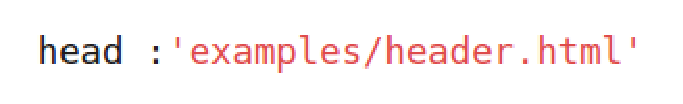
\includegraphics[width=0.4\textwidth]{images/header.eps}
  \caption{C\'odigo para incluir un header personalizado}
  \label{fig:header}
  \end{center}
  \end{figure}
  
  \begin{figure}[!th]
  \begin{center}
  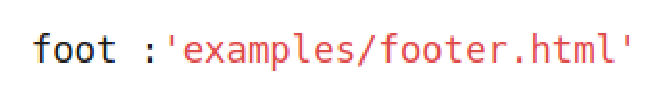
\includegraphics[width=0.4\textwidth]{images/footer.eps}
  \caption{C\'odigo para incluir un footer personalizado}
  \label{fig:footer}
  \end{center}
  \end{figure}

  \item Los textos de las preguntas admiten ahora caracteres HTML escapados usando el m\'etodo \textit{escape}.
  \begin{figure}[!th]
  \begin{center}
  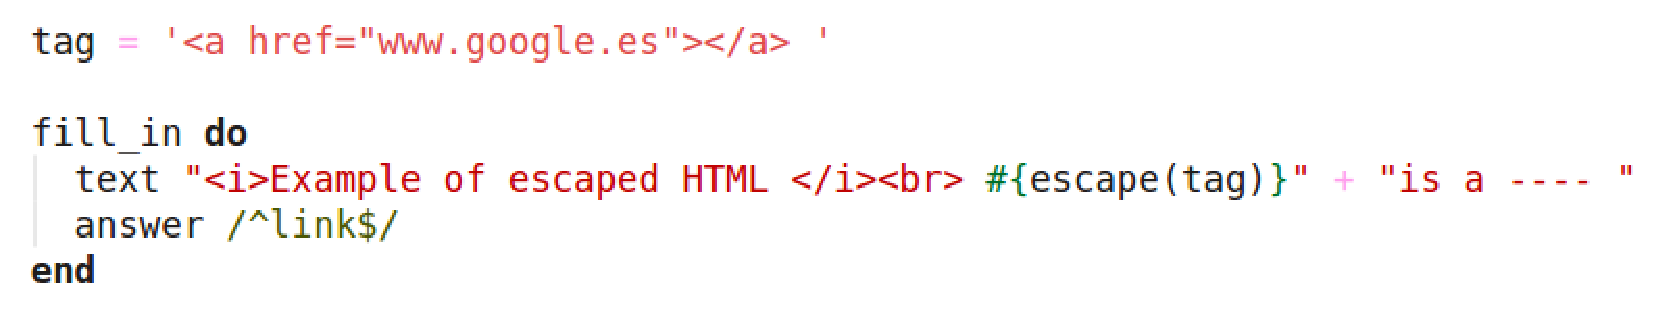
\includegraphics[width=1\textwidth]{images/tag.eps}
  \caption{Ejemplo de pregunta con HTML escapado}
  \label{fig:tag}
  \end{center}
  \end{figure}
  \newpage
  
  \item El cuestionario es capaz de renderizar expresiones escritas en {\bfseries LaTeX}.
  \begin{figure}[H]
  \begin{center}
  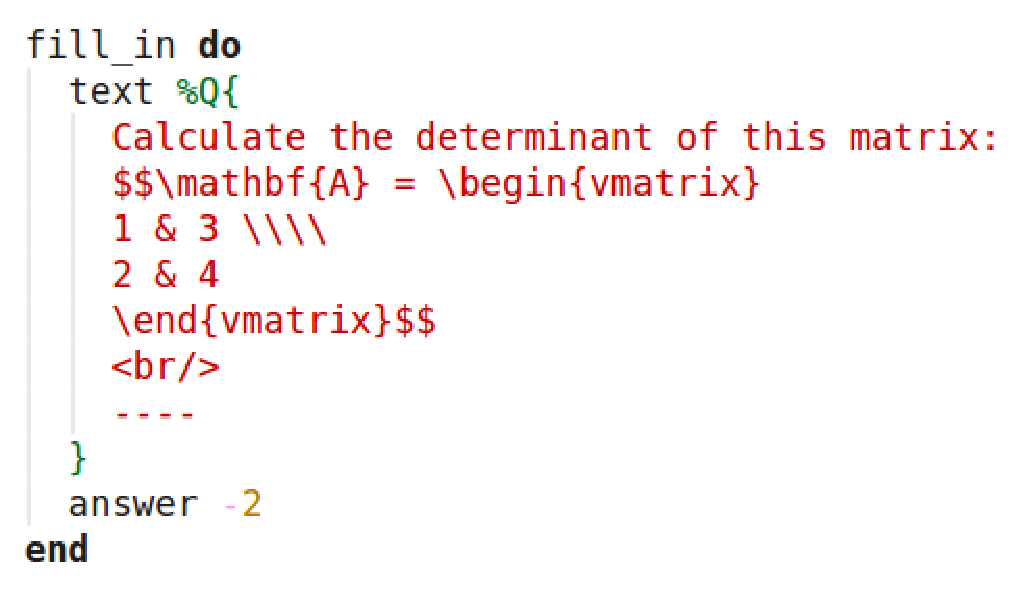
\includegraphics[width=0.6\textwidth]{images/latex.eps}
  \caption{Ejemplo de pregunta con c\'odigo LaTeX}
  \label{fig:latex}
  \end{center}
  \end{figure}
  
  \begin{figure}[H]
  \begin{center}
  
\includegraphics[width=0.8\textwidth]{images/latex2.eps}
  \caption{Ejemplo de pregunta con c\'odigo LaTeX renderizada}
  \label{fig:latex2}
  \end{center}
  \end{figure}
  \newpage
  
  \item Las preguntas de completar permiten ahora respuestas n\'umericas y de c\'odigo JavaScript.
  \begin{figure}[!th]
  \begin{center}
  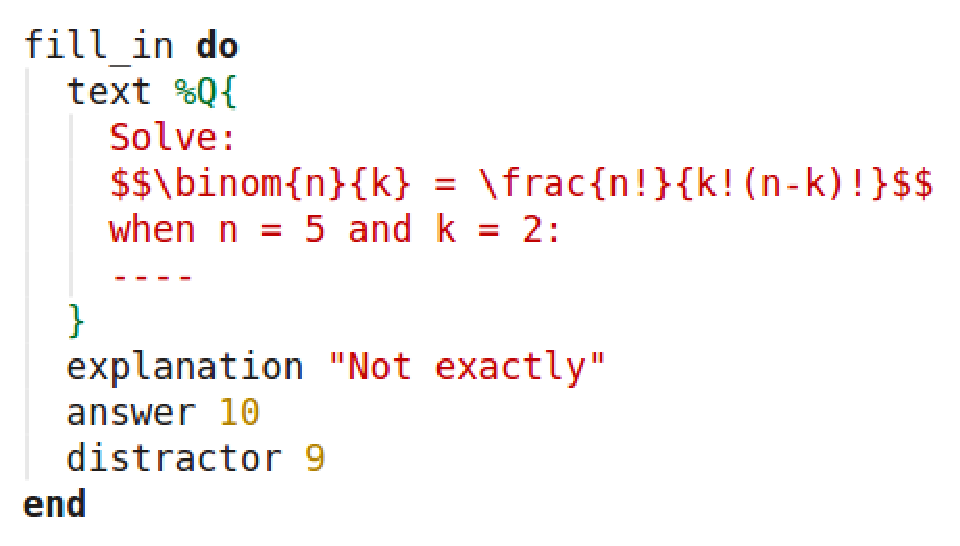
\includegraphics[width=0.6\textwidth]{images/numeric_answer.eps}
  \caption{Ejemplo de pregunta con respuesta num\'erica}
  \label{fig:numeric_answer}
  \end{center}
  \end{figure}
  
  \begin{figure}[!th]
  \begin{center}
  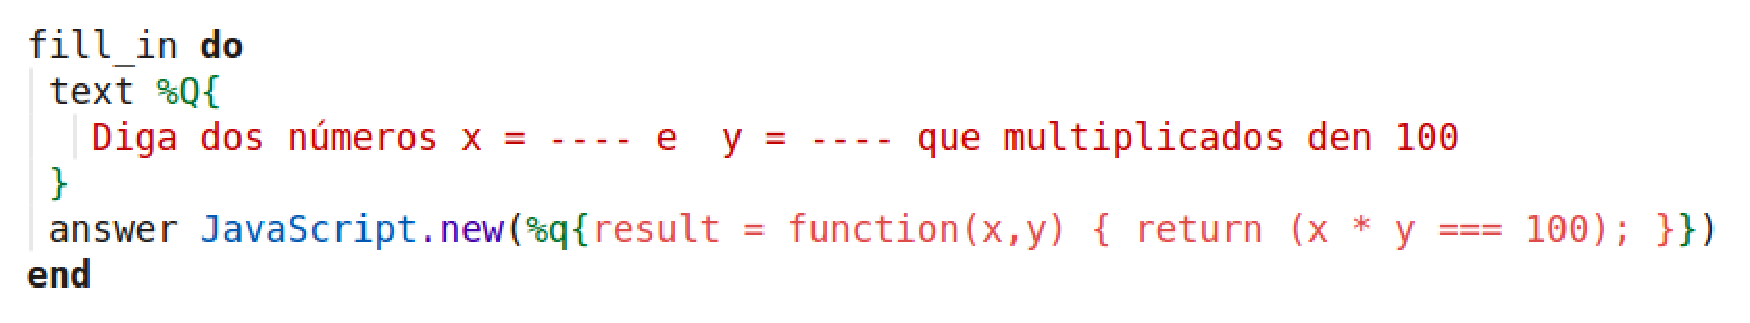
\includegraphics[width=1\textwidth]{images/javascript_answer.eps}
  \caption{Ejemplo de pregunta con respuesta de tipo JavaScript}
  \label{fig:javascript_answer}
  \end{center}
  \end{figure}
  
  \item Las espacios para rellenar las respuestas de las preguntas de completar se ajustan al tama\~{n}o de dicha respuesta.
  Para ello basta especificar tantos guiones '-' como caracteres contenga la respuesta en el fichero Ruby. Es necesario un m\'{\i}nimo
  de tres guiones, de lo contrario, no se traducir\'an dichos guiones a etiquetas input HTML.
  En caso de querer mostrar mas de tres guiones sin que sean traducidos a inputs, se deben escapar usando un \textit{backslash} ('\textbackslash')
  \begin{figure}[!th]
  \begin{center}
  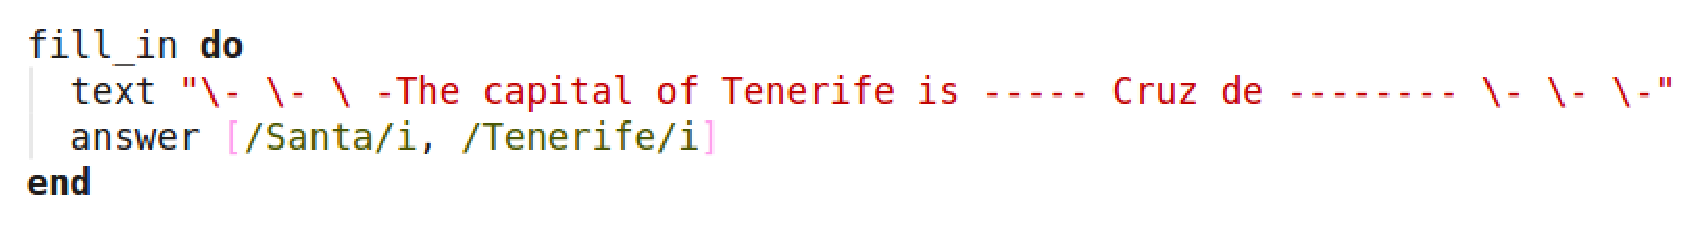
\includegraphics[width=1\textwidth]{images/input.eps}
  \caption{Ejemplo de pregunta con respuestas de m\'ultiples longitudes}
  \label{fig:input}
  \end{center}
  \end{figure}
  \newpage
  
  \begin{figure}[!th]
  \begin{center}
  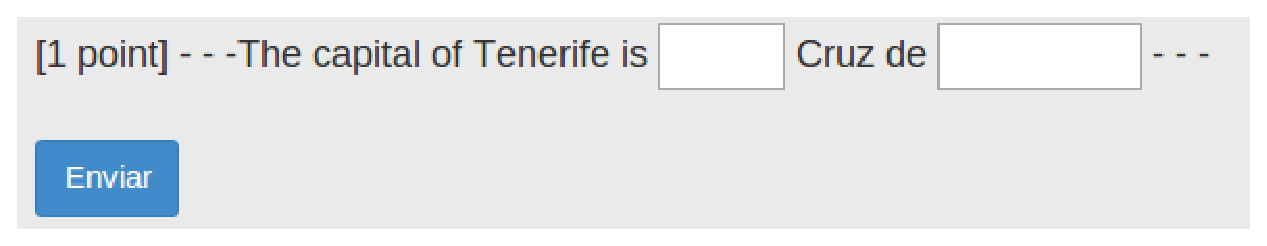
\includegraphics[width=0.8\textwidth]{images/input2.eps}
  \caption{Ejemplo de pregunta con respuestas de m\'ultiples longitudes renderizada}
  \label{fig:input2}
  \end{center}
  \end{figure}
  
  \item Cuando en una pregunta existen numerosos huecos para escribir respuestas, en el array de respuestas podr\'a haber alguna de ellas que no mantiene
  su correspondencia con el \'{\i}ndice que ocupa, por lo que se han a\~{n}adido dos nuevas maneras simplificadas de escribir estas preguntas de completar:
  \begin{itemize}
    \item Colocando la respuesta de la pregunta junto a sus guiones correspondiente. Para este tipo de escritura, solo se admiten respuestas de tipo \textit{String}.
    \begin{figure}[!th]
    \begin{center}
    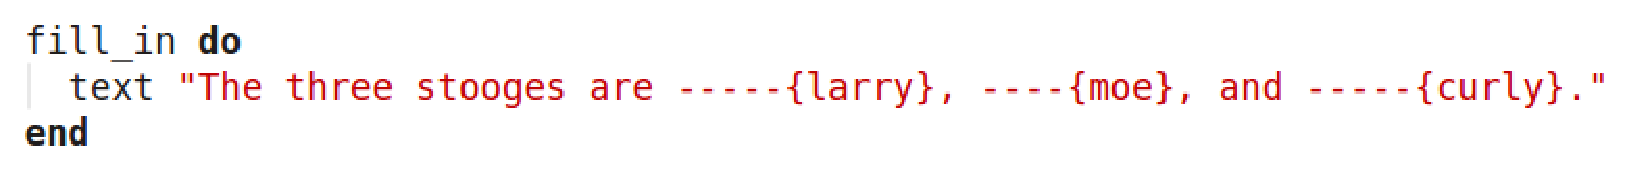
\includegraphics[width=1\textwidth]{images/simplificated1.eps}
    \caption{Ejemplo del primer tipo de pregunta simplificada}
    \label{fig:simplificated1}
    \end{center}
    \end{figure}
    
    \item Usando una notaci\'on de \textit{Hash}: especificando una clave seguida de los guiones de la respuesta y definir su correspondencia en el m\'etodo definido
    para escribir la respuesta.
    \begin{figure}[!th]
    \begin{center}
    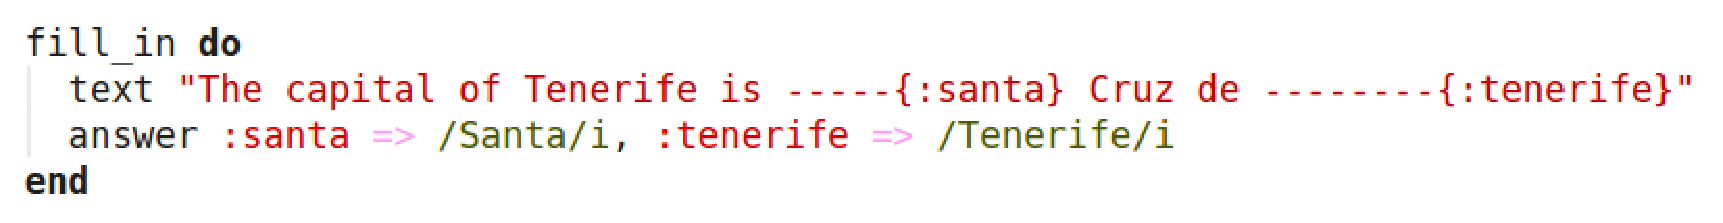
\includegraphics[width=1\textwidth]{images/simplificated2.eps}
    \caption{Ejemplo del segundo tipo de pregunta simplificada}
    \label{fig:simplificated2}
    \end{center}
    \end{figure}
    
  \end{itemize}
  \newpage
  
  \item Se han a\~{n}adido dos nuevos tipos de preguntas:
  \begin{itemize}
    \item Preguntas de {\bfseries Drag and Drop}: para preguntas de completar y preguntas tipo test (de respuesta \'unica
    y multirrespuesta).
    \begin{figure}[!th]
    \begin{center}
    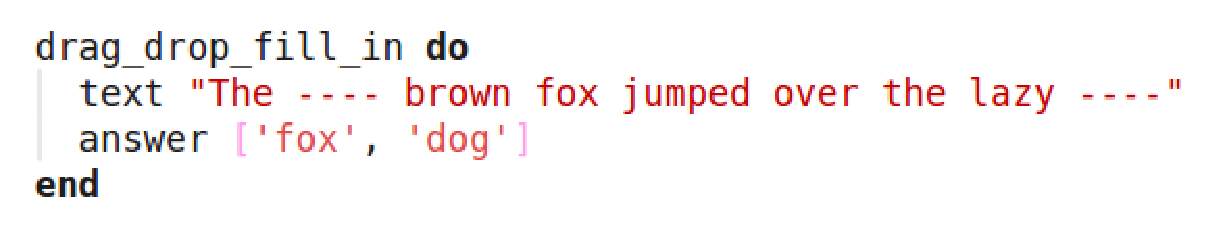
\includegraphics[width=0.8\textwidth]{images/dd1.eps}
    \caption{Ejemplo de pregunta de completar con Drag and Drop}
    \label{fig:dd1}
    \end{center}
    \end{figure}
    
    \begin{figure}[!th]
    \begin{center}
    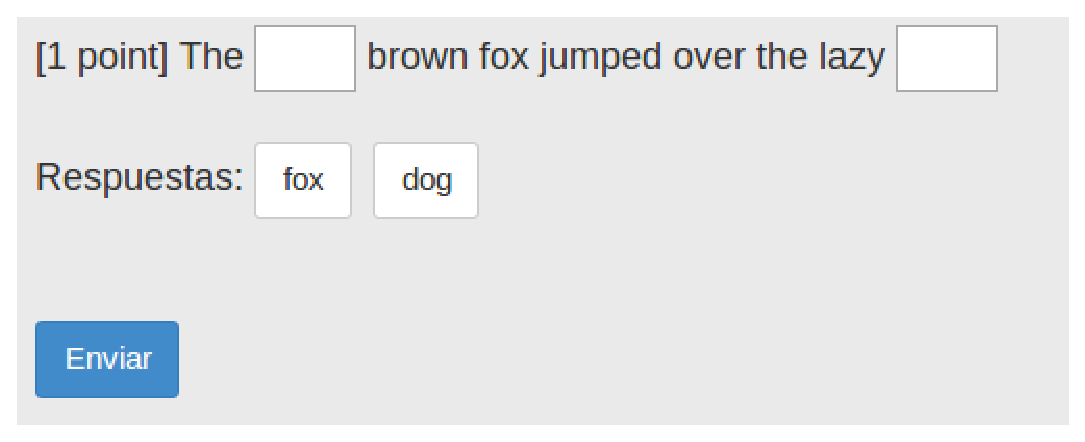
\includegraphics[width=0.8\textwidth]{images/dd1r.eps}
    \caption{Ejemplo de pregunta de completar con Drag and Drop renderizada}
    \label{fig:dd1r}
    \end{center}
    \end{figure}
    \newpage
    
    \begin{figure}[!th]
    \begin{center}
    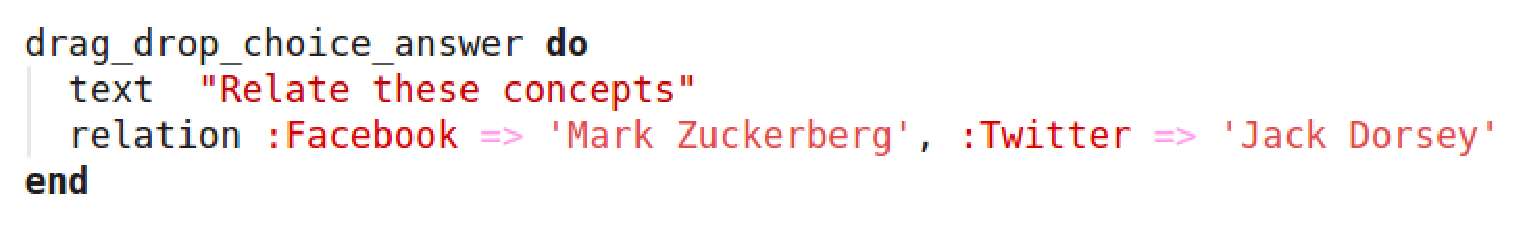
\includegraphics[width=1\textwidth]{images/dd2.eps}
    \caption{Ejemplo de pregunta tipo test de respuesta \'unica con Drag and Drop}
    \label{fig:dd2}
    \end{center}
    \end{figure}
    
    \begin{figure}[!th]
    \begin{center}
    
\includegraphics[width=1\textwidth]{images/dd2r.eps}
    \caption{Ejemplo de pregunta tipo test de respuesta \'unica con Drag and Drop renderizada}
    \label{fig:dd2r}
    \end{center}
    \end{figure}
    \newpage
    
    \begin{figure}[!th]
    \begin{center}
    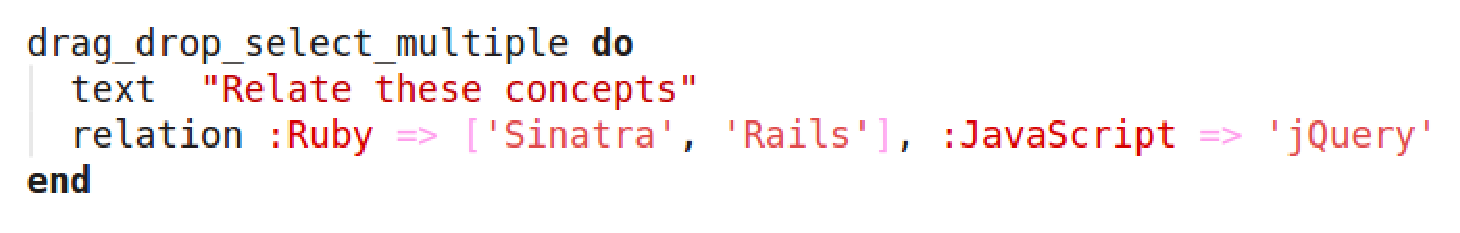
\includegraphics[width=1\textwidth]{images/dd3.eps}
    \caption{Ejemplo de pregunta de tipo test multirrespuesta con Drag and Drop}
    \label{fig:dd3}
    \end{center}
    \end{figure}
   
    \begin{figure}[!th]
    \begin{center}
    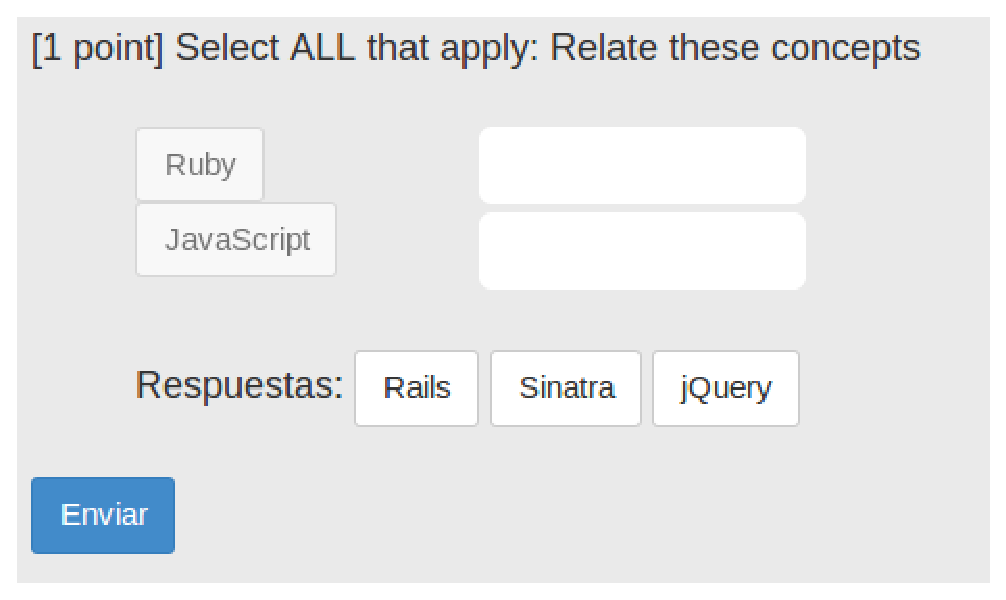
\includegraphics[width=0.6\textwidth]{images/dd3r.eps}
    \caption{Ejemplo de pregunta de tipo test multirrespuesta con Drag and Drop renderizada}
    \label{fig:dd3r}
    \end{center}
    \end{figure}
    
    {\bfseries NOTA}: en este \'ultimo tipo de pregunta Drag and Drop, la longitud del contenedor donde se insertan las 
    respuestas es el m\'aximo de la suma de las longitudes de las respuestas correctas.
    \bigskip
    
    \item Preguntas de {\bfseries programaci\'on}:
    \begin{itemize}
      \item Este tipo de preguntas s\'olo admite c\'odigo JavaScript debido a que la correcci\'on de preguntas tambi\'en 
      tiene lugar en el navegador cliente.
      \item La respuesta asignada a este tiempo de preguntas debe ser un c\'odigo JavaScript que valide la respuesta introducida
      por el alumno. Este c\'odigo puede escribirse en notaci\'on de \textit{string} o especificar el path donde se encuentra el
      fichero que contiene dicho c\'odigo.
      
      \begin{figure}[!th]
      \begin{center}
      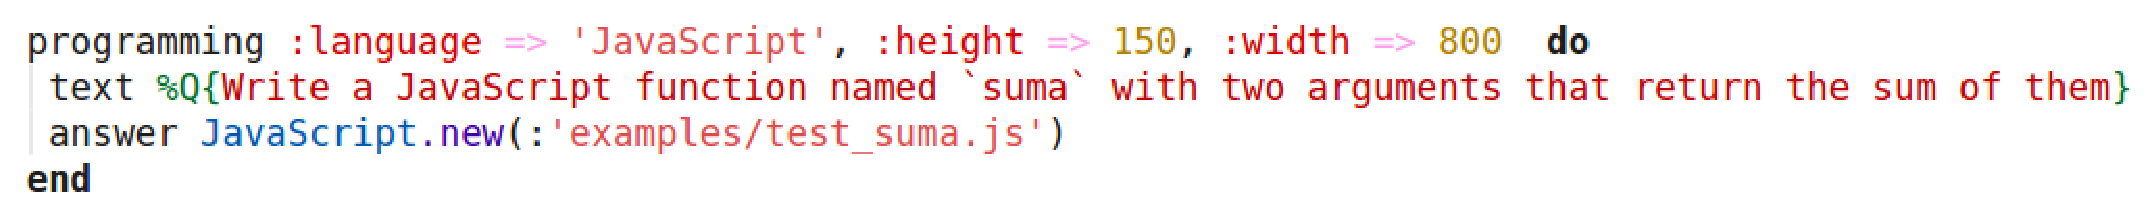
\includegraphics[width=1.1\textwidth,height=0.1\textwidth]{images/programming1.eps}
      \caption{Ejemplo de pregunta de programaci\'on}
      \label{fig:programming1}
      \end{center}
      \end{figure}
      \newpage
      
      \item Se crear\'a un \textit{textarea} de unas dimensiones definidas por defecto que tambi\'en se pueden personalizar
      y se colorear\'a el c\'odigo escrito para facilitar su lectura.
      
      \begin{figure}[!th]
      \begin{center}
      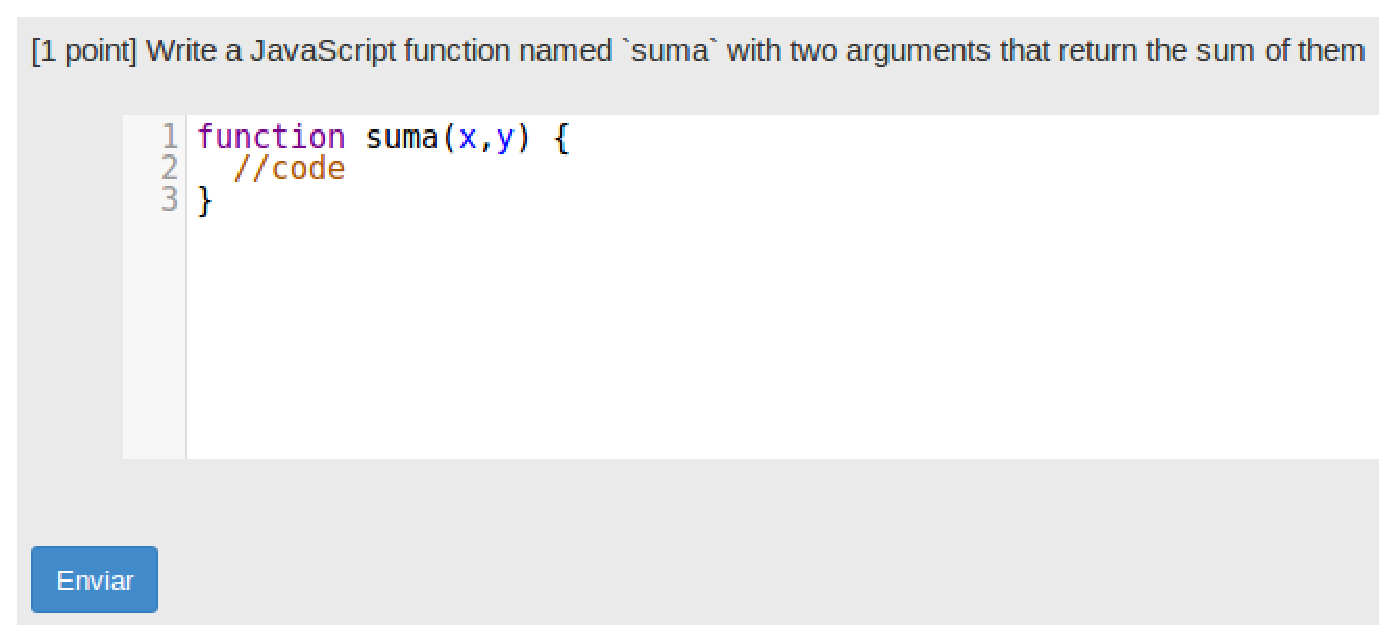
\includegraphics[width=0.9\textwidth]{images/programming1r.eps}
      \caption{Ejemplo de pregunta de programaci\'on renderizada}
      \label{fig:programming1r}
      \end{center}
      \end{figure}
      
    \end{itemize}
  \end{itemize}
  
  \item Validaci\'on autom\'atica mediante JavaScript de las preguntas que han sido rellenadas. Para corregir respuestas de tipo \textit{Regexp}
  se utiliza {\bfseries XRegExp}, mucho m\'as potente que las expresiones regulares proporcionadas en JavaScript nativo. Esta validaci\'on muestra:
  \begin{enumerate}
    \item La nota obtenida en esa pregunta.
    \item La explicaci\'on asociada a esa respuesta (si se ha especificado en el fichero Ruby).
    \begin{figure}[!th]
    \begin{center}
    
\includegraphics[width=0.7\textwidth]{images/validation1.eps}
    \caption{Ejemplo de pregunta corregida}
    \label{fig:validation1}
    \end{center}
    \end{figure}
    \newpage
    
    \item La puntiaci\'on total al final de la p\'agina.
    \begin{figure}[!th]
    \begin{center}
    
\includegraphics[width=0.9\textwidth]{images/validation2.eps}
    \caption{Puntuaci\'on total}
    \label{fig:validation2}
    \end{center}
    \end{figure}
    
  \end{enumerate}
  
  \item Almacenamiento local de las respuestas introducidas usando {\bfseries Local Storage} de HTML5.
  \item Men\'u contextual al hacer click derecho sobre el campo de respuesta para ver la respuesta correcta de dicha pregunta.
  Esta funcionalidad s\'olo est\'a disponible para preguntas de completar, cuyas respuestas sean \textit{strings},
  \textit{regexps} o num\'ericas.
  
  \begin{figure}[!th]
  \begin{center}
  
\includegraphics[width=0.8\textwidth]{images/show_answer.eps}
  \caption{Ejemplo de mostrar respuesta correcta en pregunta de completar}
  \label{fig:show_answer}
  \end{center}
  \end{figure}
  \newpage
  
  Para las preguntas tipo test existe un bot\'on que marca las respuestas correctas.
  
  \begin{figure}[!th]
  \begin{center}
  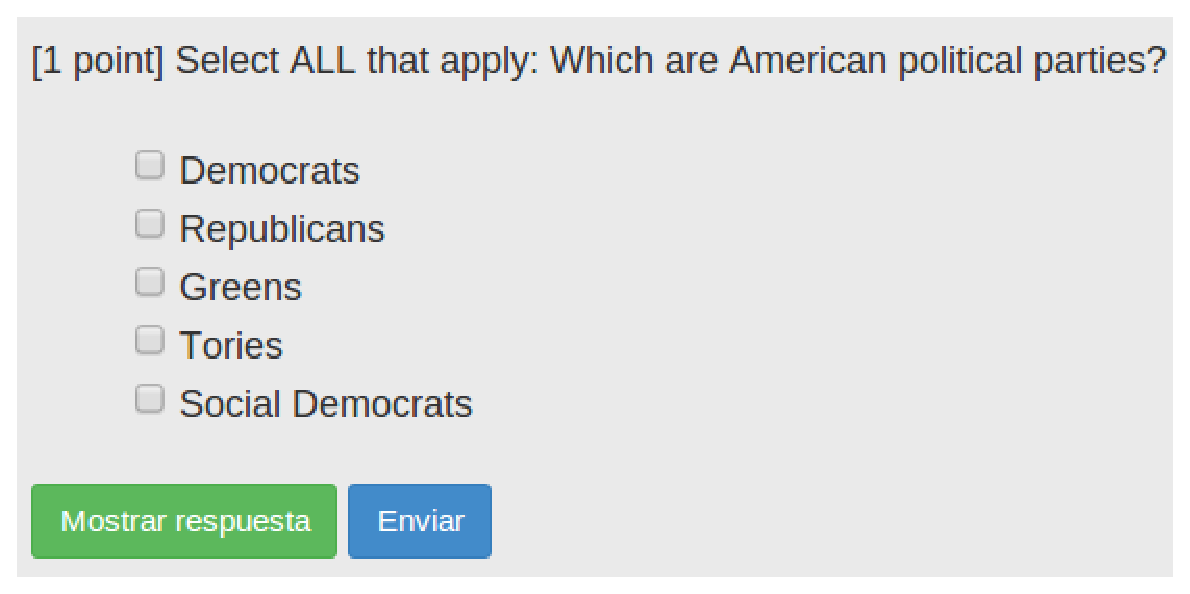
\includegraphics[width=0.65\textwidth]{images/show_answer1.eps}
  \caption{Ejemplo de mostrar respuesta correcta en pregunta tipo test}
  \label{fig:show_answer1}
  \end{center}
  \end{figure}
  
  \item Internacionalizaci\'on: la gema comprueba el idioma del sistema para ofrecer la traducci\'on adecuada al idioma del usuario
  de diversos mensajes como la correcci\'on de cada pregunta (correcto/incorrecto) o la alerta que anuncia que se ha borrado el
  Local Storage.
  Actualmente solo soporta ingl\'es y espa\~{n}ol. Para cualquier otro idioma, se utiliza el ingl\'es por defecto.
  
  \begin{figure}[!th]
  \begin{center}
  
\includegraphics[width=0.7\textwidth]{images/i18n.eps}
  \caption{Mensaje en espa\~{n}ol de Local Storage borrado}
  \label{fig:i18n}
  \end{center}
  \end{figure}

\end{itemize}
\newpage

%---------------------------------------------------------------------------------
\section{Problemas encontrados y soluciones}
\label{4:sec:1}

\subsection{Correcci\'on de preguntas de Ruby en JavaScript}
\label{subsec:4.1.2}
\bigskip

Se ha tratado de usar {\bfseries Opal} para traducir preguntas escritas en Ruby a JavaScript y poder validarlas desde el navegador.
Se consigui\'o en parte, pues no fue posible obtener el c\'odigo de una \textit{Lambda} o un \textit{Proc}, ya que Ruby los evaluaba antes de llegar al
JavaScript.
\bigskip

{\normalsize {\bfseries Soluci\'on}}
\bigskip

Permitir solamente preguntas de c\'odigo JavaScript en este renderer.

\subsection{Alojar librer\'{\i}a MathJax en un directorio de la gema}
\label{subsec:4.1.3}
\bigskip

Todos los JavaScript y CSS de terceras partes se encuentran alojadas en un directorio denominado \textit{vendor}. Para los JavaScripts y CSS
propios existe otro directorio llamado \textit{public}. Estos ficheros se insertan en el HTML generado, de modo que no es necesario manejar varios
ficheros junto con el HTML. 

Sin embargo, el framework {\bfseries MathJax}, usado para insertar texto en LaTeX en el HTML, no se ha podido insertar en el mismo. Consta de un
amplio n\'umero de ficheros y cada uno de ellos es una dependecia de otro. Adem\'as, existen numerosas im\'agenes por lo que no ha sido posible insertarlo
en el HTML de salida.
\bigskip

{\normalsize {\bfseries Soluci\'on}}
\bigskip

Hacer uso de un {\bfseries CDN} para utilizar este framework.
